\section{Background} \label{sec-background}

\subsection{Hyperparameter Optimization and AutoML}\label{background-hyperparameter-optimization}
In this section, we provide an overview of hyperparameter optimization techniques. 
Specifically, we first describe the grid search method.
Then we describe more advanced optimization methods and their heavy reliance on defining a proper search space and many iterations of search to acquire enough points to suggest good hyperparameter settings.
\subsubsection{Grid Search}
In the grid search approach, the user first defines a grid of hyperparameter values (1 dimension for every hyperparameter of the model).
The search process then proceeds to use the values at each point of the grid, trains a model to the completion, and stores the quality metrics of the model.
After executing the training operation for every point in the grid, the model with the best quality metric is chosen as the final model.
\subsubsection{Random Search}
\subsubsection{Bayesian Hyperparameter Optimization}
\subsubsection{AutoML}

\subsection{Experiment Database}
A brief overview of the experiment databases, including several prior works such as OpenML and Schelter's  ML metadata management.
OpenML and ...

%\subsection{Graph Representation of the Experiment Database}
%Description of how we will transform the experiment database into a graph.
%Figure \ref{fig-graph-creation} shows the process of converting the experiment database into a graph.
%
%\begin{figure}
%\centering
%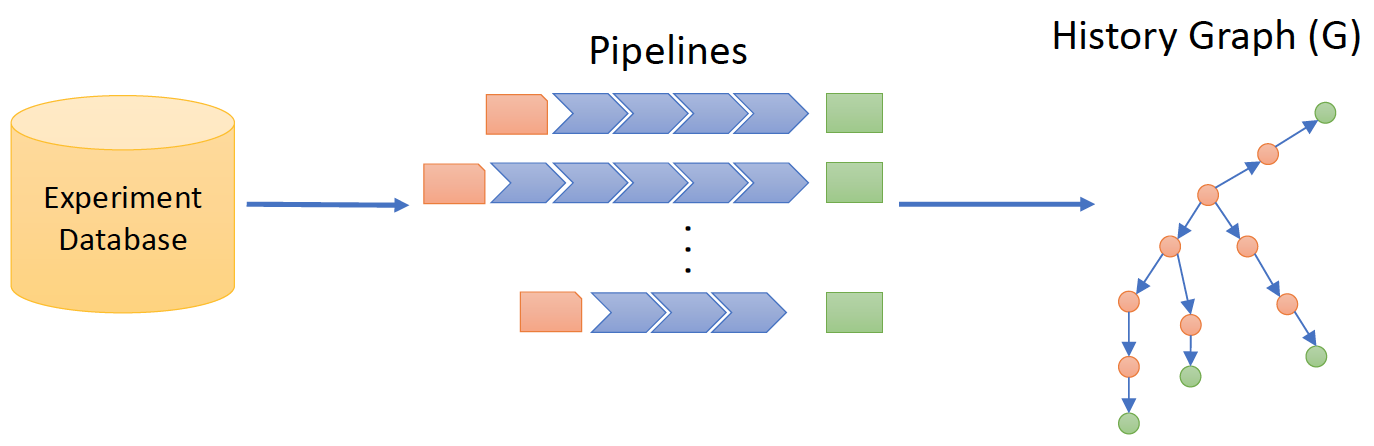
\includegraphics[width=\columnwidth]{../images/graph-creation.png}
%\caption{Process of converting the experiment database to a graph}
%\label{fig-graph-creation}
%\end{figure}
